% !TEX spellcheck = en_US

\documentclass[conference]{IEEEtran}
\usepackage{cite}
\usepackage{amsmath,amssymb,amsfonts}
\usepackage{algorithmic}
\usepackage{graphicx}
\usepackage{textcomp}
\usepackage{xcolor}
\usepackage{colortbl}
% add hyperlinks, delete all .aux files if adding hyperref after previous build
\usepackage{hyperref}
% support for unicode charcters like "é" and "ñ"
\usepackage[T1]{fontenc}
% Provides generic commands \degree, \celsius, \perthousand, \micro and \ohm
\usepackage{gensymb}
% splits a section into multiple columns
\usepackage{multicol}
\def\BibTeX{{\rm B\kern-.05em{\sc i\kern-.025em b}\kern-.08em
    T\kern-.1667em\lower.7ex\hbox{E}\kern-.125emX}}
\begin{document}

\title{Validation of Subhourly Clipping Loss Error Corrections}

\author{\IEEEauthorblockN{Abhishek Parikh\textsuperscript{1}, Kevin Anderson\textsuperscript{2}, Kirsten Perry\textsuperscript{2}, William B. Hobbs\textsuperscript{3}, Rounak Kharait\textsuperscript{1} and Mark A. Mikofski\textsuperscript{1}}
	\IEEEauthorblockA{\textsuperscript{1}DNV, San Diego, CA, 92123, USA }
    \IEEEauthorblockA{\textsuperscript{2}NREL, Golden, CO, 80401, USA }
    \IEEEauthorblockA{\textsuperscript{3}Southern Company, Birmingham, AL, 35203, USA }}

\maketitle

\begin{abstract}
Under-performance of solar PV systems is an important issue that increases risks for stakeholders like developers, investors and operators. Recently some attention has focused on underestimation of inverter clipping losses as a possible source of over-prediction where sub-hourly solar variability is high. Several models and data sets have been analyzed over the past few years, with the aim of quantifying, predicting, and correcting underestimated clipping loss errors for sites with high DC/AC ratio and solar variability. In this report, we compare operational data with a machine learning model developed at NREL to correct energy assessments based on hourly weather. In addition, the model is expanded to include site-specific information such as DC/AC ratio and modeled PV power as factors, so that the model is flexible enough to be used for estimating clipping loss error in energy assessments for a wide variety of sites. 
\end{abstract}

\begin{IEEEkeywords}
inverter, clipping, solar, irradiance, variability, performance, modeling, TMY
\end{IEEEkeywords}

\section{Introduction}
In its report "2020 Solar Risk Assessment" \cite{Matsui2020}, kWh Analytics warned that systematic underproduction across the industry exposes investors to increased risk. DNV found that a sample of 39 projects from 2019 were under-performing compared to their pre-construction energy assessments by up to 3\% on average, as shown in Fig.~\ref{fig:project-underperformance}. NextEra estimates that sub-hourly solar resource variability can affect actual energy production by approximately 1-4\%. Cormode, \textit{et al.}, explained that energy assessments based on hourly weather, like typical meteorological year (TMY) data-sets, underestimate inverter clipping losses by up to 5\% for projects with intra-hourly solar variability, especially for high DC/AC ratios \cite{Cormode2019}. This is demonstrated in Fig.~\ref{fig:irradiance-and-power}, which shows irradiance and power output at 1-minute and 1-hour resolution in the top and bottom panels, respectively. On July 10th, there is little intra-hour variability, indicative of a mostly clear day where hourly and sub-hourly simulations are in close agreement. In contrast, July 13th has much higher solar variability, but no clipping is observed in the 1-hour output. However, the 1-minute resolution shows intermittent clipping all day long, indicating that not all of the available irradiance is used by the system, and the hourly simulations underestimate inverter clipping \cite{Kharait}.

% what does the team think about citing (non-peer-reviewed) PVPMC posters? one or more of the posters that Jon Allen has presented (with me, sometimes EPRI) could be worth citing. 

\begin{figure}[htbp]
\centerline{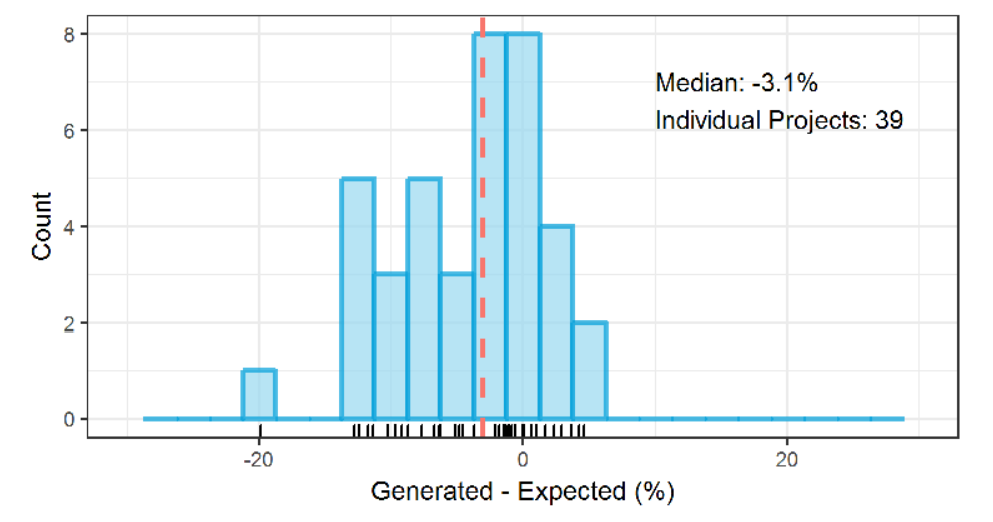
\includegraphics[width=9cm]{fig1.png}}
\caption{Project-average validation results for solar energy assessments. Each project-year was adjusted for interannual variability by scaling production by the ratio of TGY to historical monthly insolation.}
\label{fig:project-underperformance}
\end{figure}


\begin{figure}[htbp]
% combining the 1- and 60-min data on the same plot might be helpful. Additionally, using a second Y axis or normalizing GHI to 1000 w/m^2 and power to dc nameplate might help.
\centerline{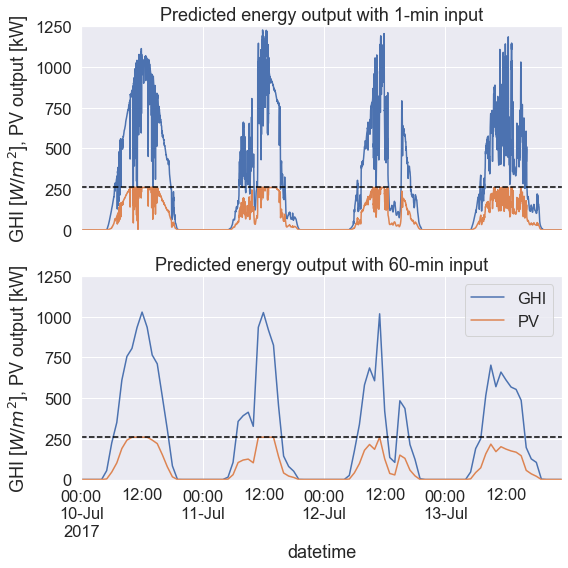
\includegraphics[width=9cm]{hourly_v_1-min_clipping.png}}
\caption{Irradiance input from the NIST test-bed weather station in Gaithersburg, MD, and predicted energy output using SolarFarmer at time-resolution of 1-minute, \textit{top panel}, and 1-hour, \textit{bottom panel}. The black dashed line in both panels shows the inverter-rated power, 260-kW.}
\label{fig:irradiance-and-power}
\end{figure}

Add description of variability index

Several methods have been proposed to correct clipping loss error in hourly predictions \cite{Cormode2019,Kharait,Anderson2020,Bradford}, but only NextEra validated their method with operational data \cite{Bradford}. 
% consider adding a reference to Hofmann 2014 (https://doi.org/10.1155/2014/808509), used in PV*SOL (see Lindemann presentation from 2017 PVPMC in ABQ, https://pvpmc.sandia.gov/resources-and-events/events/2017-8th-pv-performance-modeling-workshop/)
In this report, we adapt the NREL machine learning-based model \cite{Anderson2020} to predict clipping loss corrections and apply them to hourly energy assessments. The adjusted energy assessment is then validated against operational data from the same site, and we report on the average and distribution of validation errors.  We have obtained data from two operating PV systems in different climates and with a range of DC/AC ratios. In this paper, we will outline our method, and present model validation results for these two systems. The final paper will present validation results from all seven sites plus the NIST ground array \cite{Boyd2017b} as a benchmark.

\section{Methods}

\subsection{Model}

The machine learning (ML) model developed at NREL has already been described in detail \cite{Anderson2020}. This model was adapted for the purpose of this research. A black-box XGBoost model was generated, with satellite data inputs, as well as features derived from these fields. In an extension of the model described in \cite{Anderson2020}, system DC/AC ratio and AC power outputs from the associated SAM model were added as continuous variable features. Specific model input parameters included the following:
\begin{itemize}
\item Min-max normalized POA, GHI, clearsky POA, clearsky GHI, and cell temperature
\item First-order differenced normalized POA
\item Difference between Clearsky POA and POA
\item System DC/AC ratio
\item Modeled AC power (taken from the SAM simulation) 
\end{itemize}
The model was trained using high quality irradiance measurements from SURFRAD \cite{Augustine2000} and 1-minute to 30-minute clipping loss errors predicted using SAM \cite{Freeman2018}. The resulting trained model is then used to make predictions at the operational sites.




\subsection{Sites}


For the validation, two operational sites in Georgia were chosen. The system parameters of the two solar sites used for validation are provided in Table~\ref{table1}. These sites were selected for their high DC/AC ratio, and 1-minute data sampling frequency.

\begin{table}[htbp]
\caption{System Parameters}
\begin{center}
\begin{tabular}{ |c|c|c| } 
\hline
& Site A & Site B \\
\hline
\cellcolor{gray}Array type & Tracking & Tracking \\
\hline
\cellcolor{gray}Array azimuth & 180$^{\circ}$ & 180$^{\circ}$\\
\hline
\cellcolor{gray}DC capacity & 27 MW & 43 MW\\
\hline
\cellcolor{gray}AC capacity & 19 MW & 30 MW \\
\hline
\cellcolor{gray}DC/AC Ratio & 1.42 & 1.43 \\
\hline
\cellcolor{gray}Ground coverage ratio & 0.3 & 0.3 \\
\hline
\end{tabular}
\end{center}
\label{table1}
\end{table}



\subsection{Validation}
A challenge in validating the clipping loss correction model is the lack of quality high-frequency irradiance measurements that are co-located with operational PV systems. Therefore this model differs from traditional approaches for model training and validation because it relies on SURFRAD measurements and SAM simulated data to train the model, but uses operational data from different sites for validation. So no holdout methods are required in validating this model because the training and validation data sets are already independent. The downside of this method is that any systematic biases in SAM are introduced into the clipping loss correction model. In future work, if a large population of high-frequency irradiance and co-located operational data are obtained, the model can be retrained holding out a subset of the data for validation. This procedure would have the benefit of incorporating any physical effects that are not captured by SAM.

Quality of operational datasets is vital to avoid disruption of validation. Data points in the operational dataset related to plant sub-performance instances are considered to be outliers from the validation's standpoint and need to be removed. However, detecting sub-performance from the inverter output is challenging. For this validation effort, the bias change is presented for both unfiltered and filtered data points. For filtering, data points that met the following criteria were removed: (1) the difference between the measured, on-site POA and the modeled POA calculated using the PSM data is less than 5\%; and (2) the difference between actual power and simulated power of a particular timestep is more than 25\%. For site A and site B, 60.5\% and 55.1\% of the data is retained after applying the data filter, respectively.

In addition, high clipping errors occur during periods in which the plant is observing DC clipping (usually corresponds to higher irradiance) and high fluctuations in the irradiance. For the purpose of this validation, the fluctuations are quantified by calculating the variability index based on \cite{Stein}. The variability index is normally defined on GHI. However, since only on-site measured POA was available, the variability index for this study was calculated and aggregated at a 30-min interval using the on-site POA measured at a 1-min frequency. Since the ML model should be correcting only those periods with such conditions, the change is split into sets of low and high variability index. Periods are divided into three sets based on their variability index: (1) Low variability index  $(\leq10)$. (2) Medium variability index  $(>10$ \& $\leq50)$. (3) High variability index $(>50)$. Table.~\ref{var_index_breakdown} shows the composition of the on-site data based on the variability index. For this validation, two complete years of operational data from site A and one complete year of operational data from site B has been used.
% is this 50% of plant nameplate, or 50% of one of the power values for the individual timestep? 
% it would be good to note the # or % of intervals that were excluded


\begin{table}[htbp]
\caption{Composition of data based on variability index}
\begin{center}
\begin{tabular}{ |c|c|c| } 
\hline
& Site A & Site B \\
\hline
\cellcolor{gray}Low variability index $(\leq10)$ & 62\% & 63\% \\
\hline
\cellcolor{gray}Medium variability index $(>10$ \& $\leq50)$ & 21\% & 20\% \\
\hline
\cellcolor{gray}High variability index $(>50)$ & 17\% & 17\% \\
\hline
\end{tabular}
\end{center}
\label{var_index_breakdown}
\end{table}


The bias in the model is used to measure the reduction in clipping loss errors from the hourly energy assessment, and to identify if there are any unknown factors that are systematically affecting the results.

\begin{itemize}
\item \textbf{Bias}: Delta between the corrected energy assessment predictions and the measured operational data. Positive bias means over-predicted energy output:
\begin{equation}
\Delta E={E_\text{predicted}} - {E_\text{measured}}\label{eq:bias}
\end{equation}
Where $E$ is the energy output.
\item \textbf{Mean bias error (MBE)}: Average of the bias. Please note that a low MBE might hide seasonal or diurnal bias:
\begin{equation}
\mathit{MBE}=\frac{\sum_{n=1}^N{\Delta_n}}{N}\label{eq:mbe}
\end{equation}
Where $n$ is a single timestep, and $N$ is the total period of time. 



%\item \textbf{Root mean squared error}: Squares of the bias are positive, preventing any cancellation of opposing errors, and give a measure of the width of the error distribution:
%\begin{equation}
%\mathit{RMSE}=\sqrt{\frac{\sum_{n=1}^N{\Delta_n^2}}{N}}\label{eq:rmse}
%\end{equation}
%\item \textbf{Mean absolute error (MAE)}: A measure of the average bias that removes any cancellation of opposing errors:
%\begin{equation}
%\mathit{MAE}=\frac{\sum_{n=1}^N{\left|\Delta_n\right|}}{N}\label{eq:mae}
%\end{equation}
%\item \textbf{Error distribution}: A histogram of the bias that ideally looks like a normal distribution, centered at zero
%\item \textbf{Temporal correlation}: A plot of the bias aggregated monthly or by hour of the day, which should have a uniform flat distribution
%\item \textbf{Auto-correlation}: A plot of the bias versus the dependent parameter. Energy output ($E$) should also have a uniform distribution
%\item \textbf{Cross-correlation}: Plots of the bias versus independent parameters like irradiance, DC/AC ratio, clearness index, \textit{etc.}. These plots should ideally have a uniform distribution
\end{itemize}


\section{Results}

30-minute NSRDB data from each site was fed into the ML model to make clipping error predictions. Model input parameters are described in the Methods section above.

It is expected that the time steps with a higher variability index should have higher clipping errors. Fig.~\ref{fig:DCS-vi-clec-heatmap} shows the heat map of average variability index and the clipping loss error correction predicted for site A, respectively.

\begin{figure}[htbp]
\centerline{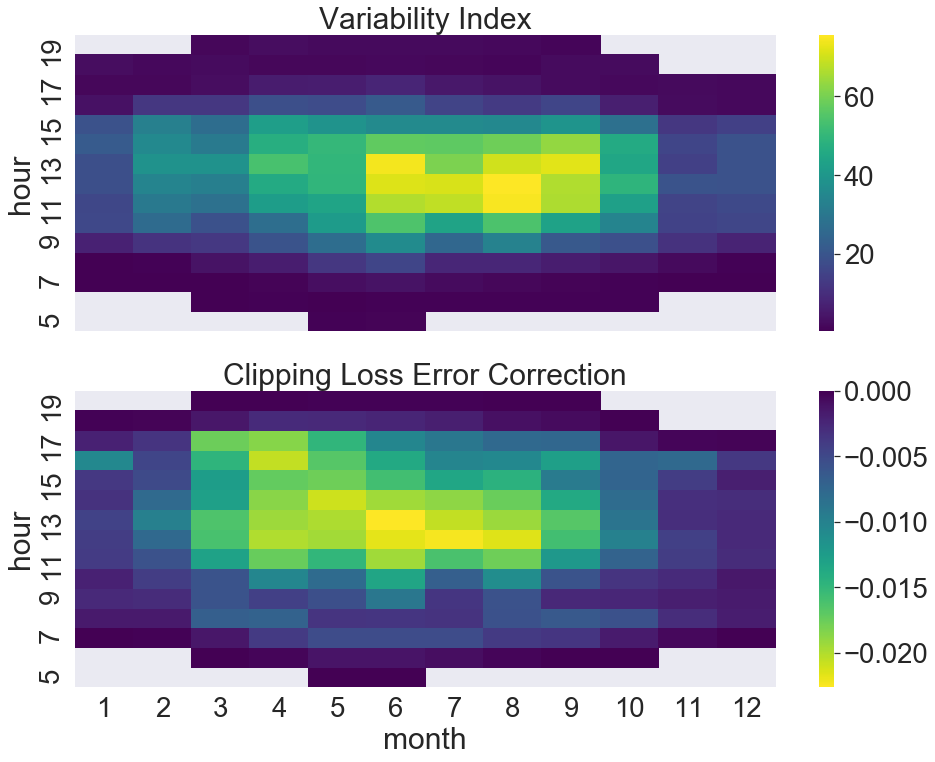
\includegraphics[width=9cm]{DCS_VI_CLEC_heatmap.png}}
\caption{The first sub-figure shows the average variability index calculated at site A. The variability index is calculated and aggregated at a 30-min interval using on-site POA measured at a 1-min time resolution. In the second sub-figure, the average clipping error correction calculated for site A using the ML model is shown. The model predicts the clipping error correction factor for each 30-min interval.}
\label{fig:DCS-vi-clec-heatmap}
\end{figure}

Fig.~\ref{fig:DCS-inv-modelbias-poa-scatter} shows the actual power of an inverter against the actual POA. At a higher variability index, the power is lower and corresponds to higher model bias.

\begin{figure}[htbp]
\centerline{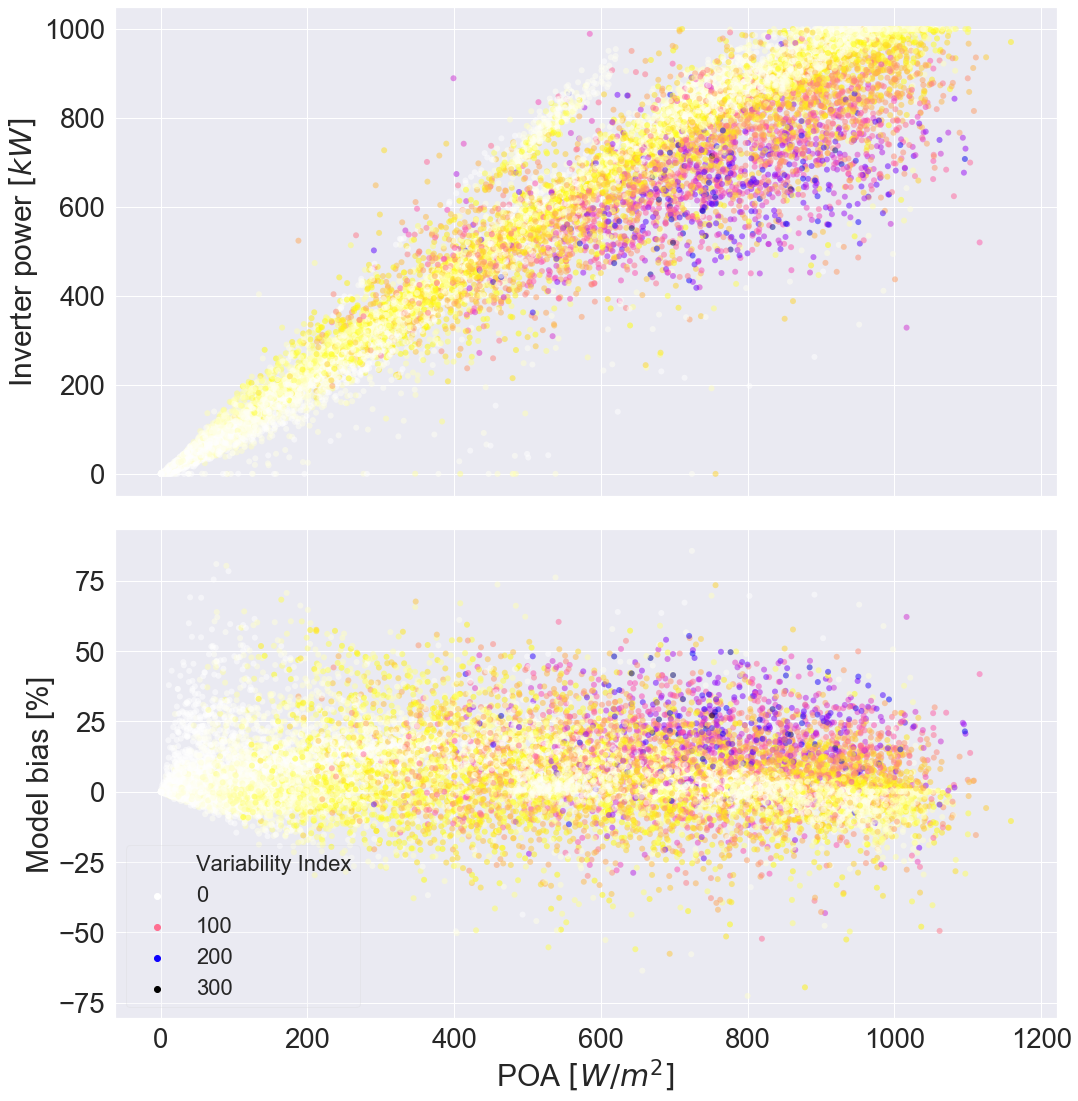
\includegraphics[width=9cm]{DCS_Inv_ModelBias_POA_with_VI.png}}
\caption{Inverter power and bias in the modeled power for a 1000 kW rated inverter at site A. Lower power and higher model bias are observed at a higher variability index}
\label{fig:DCS-inv-modelbias-poa-scatter}
\end{figure}

For the energy model, 30-minute NSRDB data was used to generate a time series of energy estimates for site A and site B. Then, these energy estimates were corrected using the clipping loss error corrections predicted by the ML model. As observed, the overall shift in the bias is small for each time series. Table.~\ref{table2} and Table.~\ref{table3} summarize the mean bias errors in the energy models before and after applying the correction, for sites A and B respectively. As indicated by Fig.~\ref{fig:DCS-vi-clec-heatmap} and Fig.~\ref{fig:DCS-inv-modelbias-poa-scatter}, the magnitude of the clipping loss error correction should be high during timesteps with high variability index and low during timesteps with low variability index. Hence, the bias is explored based on low, medium and high variability index. 

\begin{table}[htbp]
\caption{Results summary for Site A}
\begin{center}
\begin{tabular}{ |c|c|c|c| } 
\hline
Metric & Before correction & After correction & \% Change\\
\hline
Overall MBE & 5.4\% & 4.8\% & -0.6\\
\hline
MBE (High VI) & 10.7\% & 9.3\% & -1.4\\
\hline
MBE (Medium VI) & 4.3\% & 3.5\% & -0.8 \\
\hline
MBE (Low VI) & 4.4\% & 4.0\% & -0.4\\
\hline
\end{tabular}
\end{center}
\label{table2}
\end{table}


\begin{figure}[htbp]
\centerline{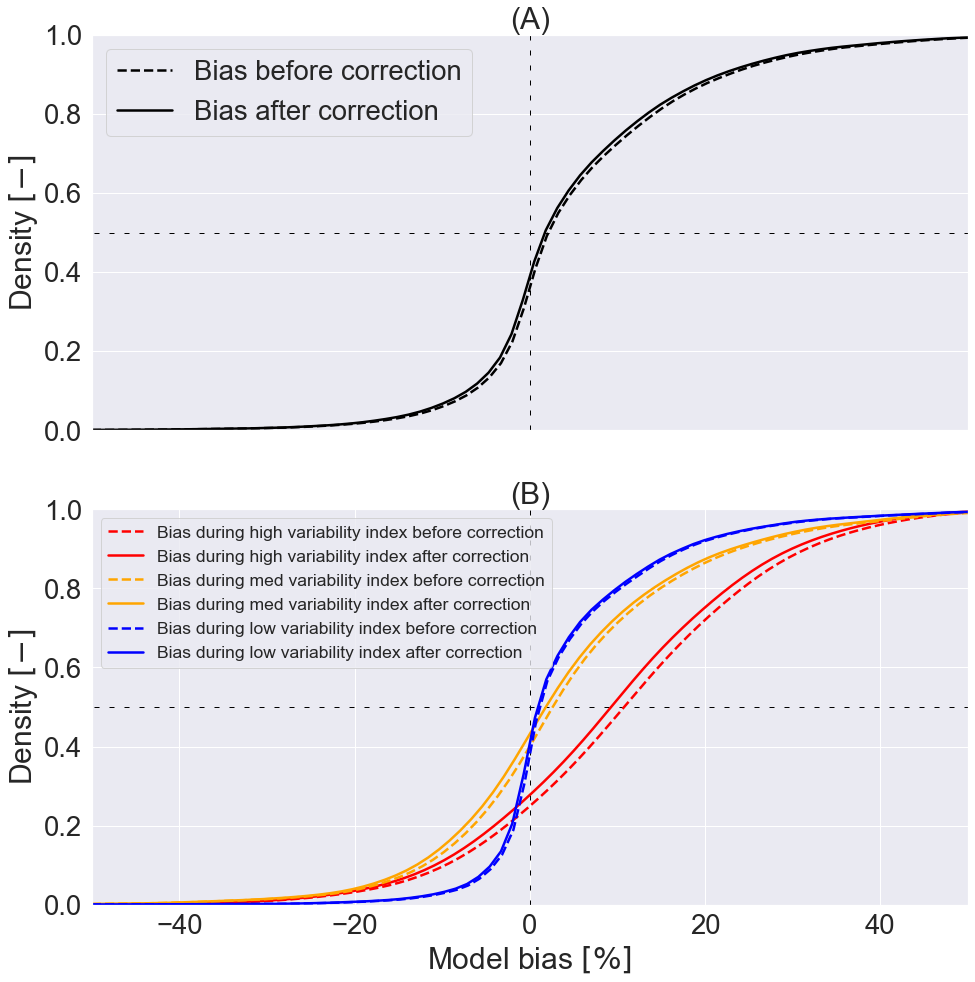
\includegraphics[width=9cm]{DCS_ModelBias_breakdown_CDF_v3.png}}
\caption{CDF of Model bias for site A before data filtering}
\label{fig:DCS-modelbias-cdf}
\end{figure}


\begin{table}[htbp]
\caption{Results summary for Site B}
\begin{center}
\begin{tabular}{ |c|c|c|c| } 
\hline
Metric & Before correction & After correction & \% Change\\
\hline
Overall MBE & 7.8\% & 6.7\% & -1.1\\
\hline
MBE (High VI) & 10.4\% & 7.9\% & -2.5\\
\hline
MBE (Medium VI) & 7.7\% & 6.3\% & -1.4\\
\hline
MBE (Low VI) & 7.1\% & 6.5\% & -0.6\\

\hline
\end{tabular}
\end{center}
\label{table3}
\end{table}

\begin{figure}[htbp]
\centerline{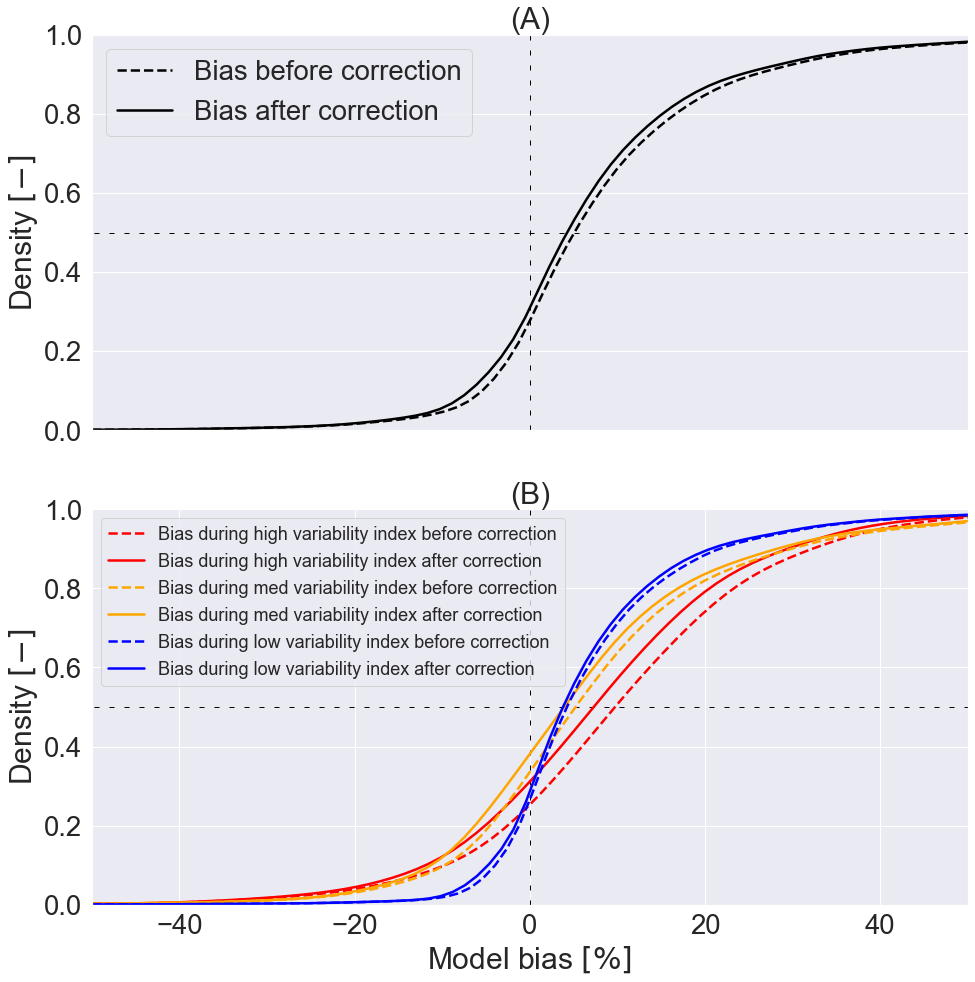
\includegraphics[width=9cm]{PAW_ModelBias_breakdown_CDF_v3.png}}
\caption{CDF of Model bias for site B before data filtering}
\label{fig:PAW-modelbias-cdf}
\end{figure}

The bias reduction for data points with high variability index is the highest compared to the data points with medium and low variability index. Overall model bias can be attributed to multiple reasons, such as the difference in the resource measured on-site and NSRDB, site specific sub-performance, incorrect loss assumption in the energy model, etc. However, for a given data point, it is unrealistic to have a bias of greater than 25\% in power when the bias in POA is less than 5\%. Consequently, points fitting this logic are removed and the bias change is recalculated.

\begin{table}[htbp]
\caption{Results summary for Site A after filtering}
\begin{center}
\begin{tabular}{ |c|c|c|c| } 
\hline
& Before correction & After correction & \% Change\\
\hline
Overall MBE & 2.3\% & 1.8\% & -0.5\\
\hline
MBE (High VI) & 10.6\% & 9.2\% & -1.4 \\
\hline
MBE (Medium VI) & 3.1\% & 2.4\% & -0.7\\
\hline
MBE (Low VI) & 1.1\% & 0.8\% & -0.3\\
\hline
\end{tabular}
\end{center}
\label{results_A_after_filter}
\end{table}

\begin{figure}[htbp]
\centerline{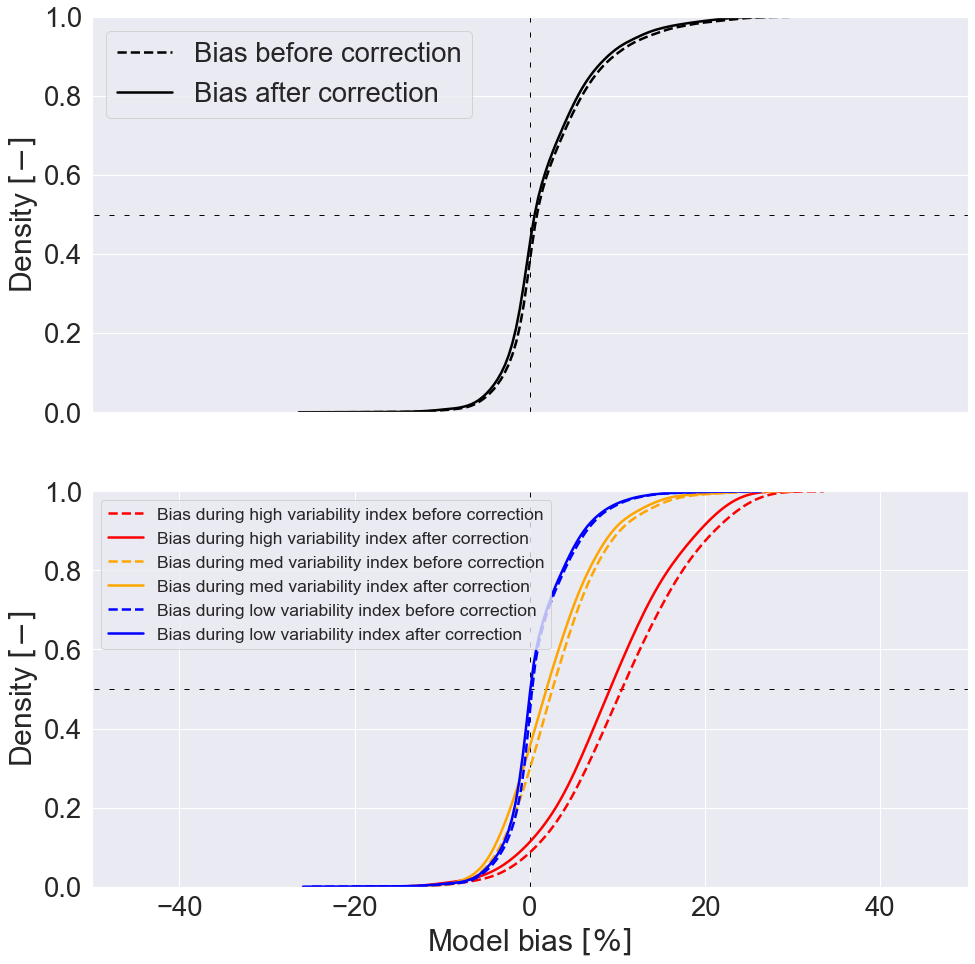
\includegraphics[width=9cm]{DCS_ModelBias_breakdown_AFTER_filter_CDF_v3.png}}
\caption{CDF of Model bias for site A after data filtering}
\label{fig:DCS-modelbias-after-filter-cdf}
\end{figure}

\begin{table}[htbp]
\caption{Results summary for Site B after filtering}
\begin{center}
\begin{tabular}{ |c|c|c|c| } 
\hline
& Before correction & After correction & \% Change\\
\hline
Overall MBE & 3.6\% & 2.8\% & -0.8\\
\hline
MBE (High VI) & 8.7\% & 6.1\% & -2.6\\
\hline
MBE (Medium VI) & 4.4\% & 3.0\% & -1.4\\
\hline
MBE (Low VI) & 2.8\% & 2.4\% & -0.4\\
\hline
\end{tabular}
\end{center}
\label{results_A_after_filter}
\end{table}

\begin{figure}[htbp]
\centerline{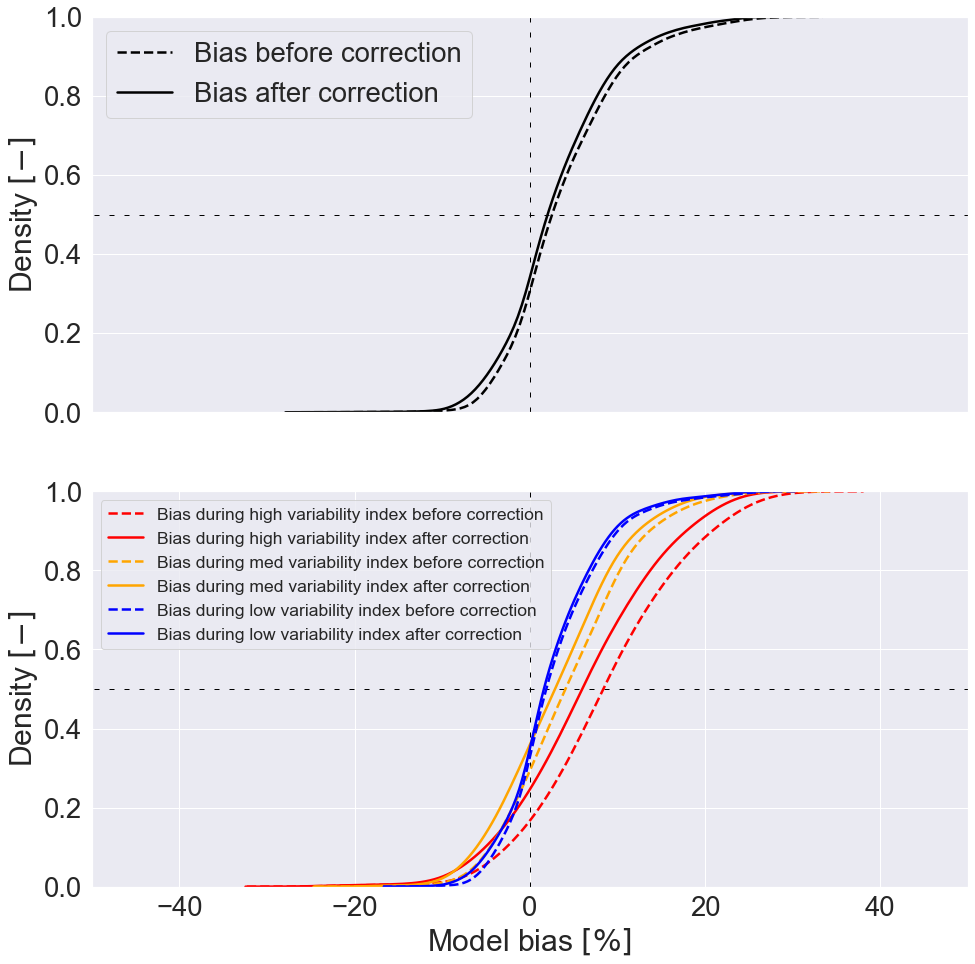
\includegraphics[width=9cm]{PAW_ModelBias_breakdown_AFTER_filter_CDF_v3.png}}
\caption{CDF of Model bias for site B after data filtering}
\label{fig:PAW-modelbias-after-filter-cdf}
\end{figure}

\section{Conclusions}
Over-prediction occurs in typical energy assessments that use hourly data if the sites have sub-hourly solar variability and high DC/AC because clipping losses are underestimated. These errors have been quantified using a machine-learning model trained on high-frequency solar irradiance data and simulated operational data to create clipping loss error corrections. The corrections were applied to a typical hourly energy assessment of an existing operational site and compared to the measured output from the same site. The mean bias error was reduced from 5.07\% to 4.54\%. 

\section*{Acknowledgment}

This work was authored in part by Alliance for Sustainable Energy, LLC, the manager and operator of the National Renewable Energy Laboratory for the U.S. Department of Energy (DOE) under Contract No. DE-AC36-08GO28308. Funding provided by the U.S. Department of Energy’s Office of Energy Efficiency and Renewable Energy (EERE) under Solar Energy Technologies Office (SETO) Agreement Numbers 34348. The views expressed in the article do not necessarily represent the views of the DOE or the U.S. Government. The U.S. Government retains and the publisher, by accepting the article for publication, acknowledges that the U.S. Government retains a nonexclusive, paid-up, irrevocable, worldwide license to publish or reproduce the published form of this work, or allow others to do so, for U.S. Government purposes.

\bibliographystyle{IEEEtran}
% argument is your BibTeX string definitions and bibliography database(s)
\bibliography{IEEEabrv,bibliography}

\end{document}
